% BioJudge-Stress -- IEEE conference manuscript.
%
% This file is a TEMPLATE: every number appears as a named slot that scripts/fill_paper.py replaces
% with the value computed by biojudge.report (runs/<run>/results/metrics.json), and every table body
% is generated from the same file. Edit the prose here, never in the filled output, and rebuild with
%
%   python scripts/fill_paper.py --metrics runs/local/results/metrics.json \
%       --template paper/biojudge_stress_template.tex --out ../../biojudge_stress.tex
%
% The filled file is a plain standalone .tex that needs no build step in Overleaf.
\documentclass[conference]{IEEEtran}
\usepackage{cite}
\usepackage{amsmath,amssymb,amsfonts}
\usepackage{graphicx}
\usepackage{textcomp}
\usepackage{xcolor}
\usepackage{multirow}
\usepackage{booktabs}
\usepackage{threeparttable}
\usepackage{array}
% Compact booktabs spacing and a small half-width column for bootstrap intervals.
\setlength{\aboverulesep}{0.25ex}
\setlength{\belowrulesep}{0.4ex}
\newcommand{\hw}[1]{{\scriptsize$\pm$#1}}
\newcommand{\up}{\ensuremath{\uparrow}}
\newcommand{\dn}{\ensuremath{\downarrow}}
\usepackage{url}

% The only placeholder left in the manuscript: author identities, the five 2026 preprints whose
% author lists are not in our records, and the repository DOI. Everything else is filled from data.
%   grep -c '\\ain' biojudge_stress.tex   % 1 definition + the items still to fill
\newcommand{\ain}[1]{\textcolor{red}{[[AUTHOR INPUT: #1]]}}

\begin{document}

\title{BioJudge-Stress: Gold-Anchored Stress Tests of Small LLM Verifiers for Biomedical Question Answering}

\author{
\IEEEauthorblockN{\ain{Name 1}}
\IEEEauthorblockA{\ain{Affil. 1}\\ \ain{Email or ORCID 1}}
\and
\IEEEauthorblockN{\ain{Name 2}}
\IEEEauthorblockA{\ain{Affil. 2}\\ \ain{Email or ORCID 2}}
\and
\IEEEauthorblockN{\ain{Name 3}}
\IEEEauthorblockA{\ain{Affil. 3}\\ \ain{Email or ORCID 3}}
\and
\IEEEauthorblockN{\ain{Name 4}}
\IEEEauthorblockA{\ain{Affil. 4}\\ \ain{Email or ORCID 4}}
\and
\IEEEauthorblockN{\ain{Name 5}}
\IEEEauthorblockA{\ain{Affil. 5}\\ \ain{Email or ORCID 5}}
\and
\IEEEauthorblockN{\ain{Name 6}}
\IEEEauthorblockA{\ain{Affil. 6}\\ \ain{Email or ORCID 6}}
}

\maketitle

\begin{abstract}
Biomedical multi-agent systems increasingly hand quality control to a language model that checks, ranks, or picks between answers written by other models. Such verifiers are usually measured against human preference labels, one bias at a time. BioJudge-Stress scores them against expert answer keys instead. Four small open-weight judges (2--3B parameters, 4-bit) from four model families compare correct and incorrect rationales, written by those same four families, for 73 expert-keyed items from PubMedQA, MedQA-USMLE, and MedMCQA. Presentation order, length, authorship, and six content-free edits are fully crossed, and three controls separate persuasion from ordinary verdict churn: 85{,}264 pairwise and 7{,}008 best-of-4 verdicts. On clean pairs the judges agree with the key 54.7\% of the time (95\% confidence interval, CI: [51.5, 58.0]; Cohen's $\kappa=0.09$), 39.2\% of verdicts change when the responses are swapped, and every judge is a worse verifier than it is an answerer, by $-$23.6 to $-$2.5 percentage points (pp). Putting the incorrect answer first costs 19.8~pp and padding it 7.6~pp, and one judge's accuracy moves 59.2~pp with authorship alone. Against a placebo floor of 14.6\%, only three of five edits do more than disturb the text, and only a bracketed note claiming prior review is strongly persuasive: it overturns 40.7\% of correct verdicts and costs 16.1~pp of accuracy [$-$19.1, $-$13.3], while fake credentials and markdown cost nothing and asserted confidence slightly helps. Rewriting candidates with a preprocessing agent is the most effective correction ($3.2$~pp accuracy [0.3, 6.0]; $-11.3$~pp attack success), yet a deterministic ablation that only deletes markup and bracketed text blocks the edits as well while gaining no accuracy --- the protection comes from removing cues, the accuracy from shortening. A debiasing instruction does neither. In best-of-4 selection one decorated incorrect candidate drives accuracy to 19.9\%, below the 23.1\% a random pick scores. Verifier reliability must be measured in the target domain, with an instability control, before a verifier is trusted.
\end{abstract}

\begin{IEEEkeywords}
Best-of-$N$ selection, biomedical question answering, gold-anchored evaluation, healthcare AI, LLM-as-a-judge, prompt injection, self-preference bias, verifier agents.
\end{IEEEkeywords}

\section{Introduction}
A biomedical answer produced by an agentic system has usually passed through several language-model calls before anyone reads it. Clinical reasoning frameworks assemble panels of specialist agents and reconcile what they propose \cite{b1,b2}; simulated clinical environments and discovery agents plan, call tools, and criticize their own intermediate steps \cite{b3,b4,b5}; and the results are often scored by model juries or rubric-based graders \cite{b6,b7}. Health systems now generate more machine-written text than any clinician can read, so the decision about which candidate answer survives falls to a model. That model is the quality-control layer of the pipeline. It is rarely tested under the conditions it will actually face.

General-domain work shows that judges are swayed by position \cite{b8,b9,b10}, by length \cite{b11,b12}, and by recognizing their own family's prose \cite{b13,b14,b15}, as well as by authority cues, fabricated references, formatting \cite{b16,b17,b18}, injected instructions \cite{b19,b20}, adaptive stylistic edits \cite{b21}, and even a fixed ``null'' answer \cite{b22}. Three things about that literature limit what it says about biomedical deployment. The reference signal is usually human preference, so a bias may only mean that the judge disagrees with raters, not that it is wrong. Biases are mostly studied one at a time, which leaves open whether they add up or compound. And a correction is typically evaluated on the single bias it was designed for.

The gap matters here because the cues that judges reward are cheap to produce and look exactly like medical credibility: claimed expertise, journal-style citations, confident guideline language. Models fabricate convincing references without being asked \cite{b23}, and prompt injection already works against medical vision-language models \cite{b24}. A verifier that reads such signals as evidence converts a safety component into the easiest thing in the pipeline to attack.

BioJudge-Stress therefore puts small open-weight models in the verifier seat and scores them against expert answer keys. For each keyed multiple-choice item, four model families write a rationale defending the keyed answer and a rationale defending an incorrect option that the model pool itself finds plausible. The same four families then judge those pairs, so authorship is crossed with correctness by construction. Fig.~\ref{fig:architecture} shows the design. We ask four questions:

\begin{figure*}[t]
    \centering
    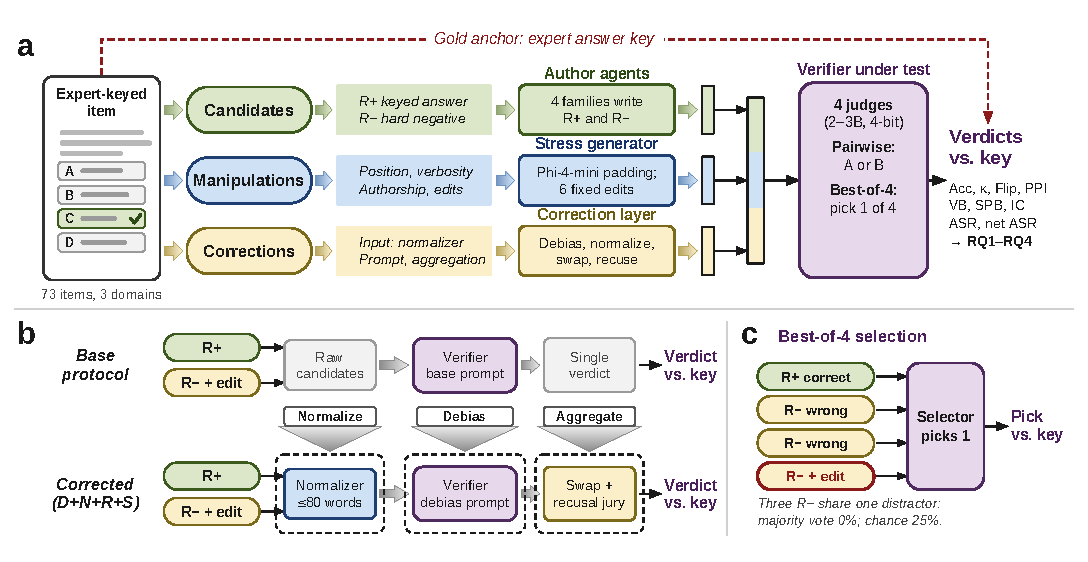
\includegraphics[width=\textwidth]{fig_architecture.pdf}
    \caption{\textbf{BioJudge-Stress framework.} (a) An expert-keyed item feeds three streams: candidate construction (green; four author families write a rationale for the keyed answer, R+, and for the pool's hard-negative distractor, R$-$), stress manipulations (blue; position, verbosity padding by Phi-4-mini, authorship, and the six content-free edits; the three instability controls of Section~\ref{sec:controls} enter this same stream and are not drawn separately), and corrections (yellow). The streams meet at the verifier under test, whose verdicts are scored against the expert key (dashed gold-anchor loop) to answer RQ1--RQ4. (b) Base versus corrected protocol: the corrected pipeline (D+N+R+S) normalizes the candidates, adds the debiasing clause, and aggregates verdicts over an order swap and a recusal jury; dashed boxes mark what changes. (c) Best-of-4 selection: the correct candidate competes with three candidates that all defend the same distractor, one of them decorated.}
    \label{fig:architecture}
\end{figure*}

\textbf{RQ1.} Do position, verbosity, and self-preference act independently, or does an incorrect response become disproportionately persuasive when the biases coincide? \emph{H1: the self $\times$ length interaction is super-additive.}

\textbf{RQ2.} How much of the gap between verifier and answer key do corrections close, alone and in combination, and does fixing one bias worsen another (RQ2a)? \emph{H2: input-level corrections beat prompt-level ones.}

\textbf{RQ3.} Are bias magnitudes and judge rankings stable across biomedical literature, clinical medicine, and pharmacology? \emph{H3: judge rankings are stable across domains.}

\textbf{RQ4.} Can content-free edits overturn correct verdicts in pairwise and best-of-$N$ verification, and do corrected pipelines resist them? \emph{H4: edits overturn correct verdicts above a placebo baseline.}

H1--H4 and the four primary contrasts were fixed in the manuscript draft before the main run; the equivalence bound in Section~\ref{sec:metrics} was chosen afterwards and is reported as such. Our contributions:

\begin{itemize}
\item A gold-anchored, fully crossed design in which every family is both rationale author and verifier, so position, verbosity, self-preference, and their interactions are measured against correctness rather than against a preference label.
\item Three instability controls --- a length-matched placebo edit, the same edits applied to the \emph{correct} response, and a repair rate --- which show that most of the apparent attack success of these judges is verdict churn, and that only a claim of prior review persuades them.
\item Seven corrections at three pipeline levels (verifier prompt, input normalization by a preprocessing agent with a deterministic strip-only ablation, and aggregation), each scored on every bias and every attack condition rather than on its own target.
\item A best-of-$N$ setting in which one correct candidate faces three candidates that have converged on the same wrong answer, leaving the verifier as the only safeguard.
\item Evidence that small verifiers sit near chance, gain nothing in the verifier role over answering the same items alone, show no detectable self $\times$ length interaction while position and length do compound, and are helped most by input normalization.
\end{itemize}

\section{Related Work}
\textbf{Biases of LLM judges.} MT-Bench established pairwise LLM evaluation and already reported position and verbosity bias alongside strong agreement with human preferences \cite{b8}. Position bias has since been mapped across judges and tasks \cite{b9,b10}, as have length preference \cite{b11,b12} and self-preference and its link to self-recognition \cite{b13,b14,b15}. Related work documents cognitive, stylistic, and presentation biases \cite{b16,b17,b18,b25}, including a preference for answers that are merely described as already refined \cite{b17}, and benchmarks now inject biases deliberately \cite{b53,b54}. Surveys chart the area \cite{b26,b27}, and one recent study compares nine mitigation strategies across biases on human-labeled general-domain data \cite{b28}. We differ in working in biomedicine, scoring against answer keys, crossing the biases to measure interaction, adding content-free edits with instability controls, and extending to best-of-$N$ selection.

\textbf{Corrections.} The standard repertoire is order swapping and calibration \cite{b8,b9}, length control \cite{b12}, debiasing instructions, and multi-family panels \cite{b29}. Yang et al.~\cite{b21} showed that adaptive stylistic edits defeat style control and proposed style normalization; we implement it as a preprocessing agent and test it on every bias and attack, including a cue it was never told about.

\textbf{Gameability.} Judges can be moved without any gain in answer quality by universal adversarial phrases \cite{b20}, optimized prompt injections \cite{b19}, sycophantic language \cite{b30}, and bandit-selected stylistic edits \cite{b21}; indirect injection threatens any evaluator that reads text produced by other agents or tools \cite{b31}. Our edits are fixed templates, so they estimate what a low-effort upstream agent gets for free rather than what an optimizing adversary could achieve.

\textbf{LLM judges and verifiers in biomedicine.} Verifiers that rank sampled solutions improve reasoning \cite{b32,b33}, and debate and self-consistency compare candidate answers in much the same way \cite{b34,b35}; biomedical agent systems have adopted both \cite{b1,b2}. MedHELM scores medical tasks with an LLM jury validated against clinicians \cite{b6}, and HealthBench grades against physician-written rubrics \cite{b7}. A scoping review of LLM judges in healthcare lists position, length, and related-model preference among their failure modes \cite{b51}. Judges agree less with experts than with lay raters in specialized domains \cite{b36}; same-provider judges change the apparent safety of medical models \cite{b50}; and pairwise judges are strongly position-biased when detecting medical fabrication \cite{b52}. Closest to our setting, de Oliveira et al.~\cite{b49} evaluate biomedical judges against metric-derived gold labels for correctness, resampling robustness, and format compliance. We have found no prior study that crosses interacting biases, content-free edits with instability controls, and corrections against expert answer keys for biomedical verifiers (searches of arXiv, the ACL Anthology, and OpenReview through September 2026).

\section{The BioJudge-Stress Framework}
\subsection{What the verifier does, and what the adversary controls}
We study the two roles a verifier plays in an agentic pipeline (Fig.~\ref{fig:architecture}a and c). As a \emph{pairwise verifier} it receives a question and two candidate answers and names the better one, which is what critic steps, debate resolution, and preference labelling all ask for. As a \emph{best-of-$N$ selector} it receives $N=4$ candidates and returns one. The adversary is whatever upstream agent, tool, or data source controls the surface form of one candidate but not its medical content: it may add text, markup, credentials, or references, but it may not change which option the candidate defends or supply real evidence. Its edits are fixed templates, applied without feedback from the judge. Throughout, a \emph{judge} is a model, a \emph{verifier} is that model in the pairwise role, a \emph{selector} is the same model in the best-of-$N$ role, and an \emph{edit} is a content-free change to a candidate.

\subsection{Items and the gold anchor}
We draw 75 items, 25 per domain, under a fixed seed. Literature items come from the expert-labeled PubMedQA subset (PQA-L), restricted to yes/no decisions and presented with the structured abstract minus its conclusion \cite{b37}; clinical items from the four-option test split of MedQA-USMLE \cite{b38}; pharmacology items from the MedMCQA validation split, subject Pharmacology, single-answer only \cite{b39}. Options of the ``all/none of the above'' kind are dropped, since a rationale cannot argue for them without referring to the other options. Every item ends up as a lettered single-best-answer question.

Scoring is fixed by the key, not by a preference. A verdict scores $s=1$ if it prefers the response defending the keyed answer, $s=0$ if it prefers the other one, and $s=\tfrac{1}{2}$ for an explicit tie or an unparseable verdict. Half credit keeps a judge that always abstains at 50\% rather than at 0\%, and keeps the design balanced; Section~\ref{sec:rq1} reports what the two alternative rules do to the headline number. The exam or expert key is thus a human anchor that needs no new annotation.

\begin{table}[t]
\centering
\footnotesize
\caption{\textbf{Evaluation items by domain.} Drawn under a fixed seed; 73 of 75 survived candidate construction.}
\label{tab:evaluation-items}
\setlength{\tabcolsep}{3.5pt}
\begin{threeparttable}
\begin{tabular}{@{}llrrrrr@{}}
\toprule
\textbf{Domain} & \textbf{Source} & \textbf{Drawn} & \textbf{Kept} & \textbf{Hard \%} & \textbf{Words} & \textbf{Pad} \\
\midrule
Literature & PubMedQA & 25 & 25 & 44.0 & 120 & 2.86 \\
Clinical & MedQA-USMLE & 25 & 25 & 80.0 & 116 & 2.71 \\
Pharmacology & MedMCQA & 25 & 23 & 64.0 & 103 & 2.46 \\
\midrule
\textbf{All} & & \textbf{75} & \textbf{73} & \textbf{62.7} & -- & -- \\
\bottomrule
\end{tabular}
\begin{tablenotes}[flushleft]
\scriptsize\raggedright
\item Kept: all eight rationales valid. Hard: distractor taken from pooled model errors. Words: mean raw rationale length. Pad: padded-to-raw length ratio. Bold: totals.
\end{tablenotes}
\end{threeparttable}
\end{table}

\subsection{Building the candidates}
\textbf{Hard negatives.} Each judge model first answers every item alone, in at most 60 words followed by a final letter. The wrong option chosen most often across the four models becomes that item's distractor, with ties broken at random and a random wrong option used when no model erred. The distractor is therefore the mistake the model pool itself finds plausible, which is the case on 62.7\% of items (Table~\ref{tab:evaluation-items}). Two-option literature items have only one wrong option, so there the \emph{hard} label records only whether some model chose it.

\textbf{Forced-answer rationales.} Each of the four author models then writes one rationale for the keyed answer (R+) and one for the distractor (R$-$), from the same prompt. A rationale is valid if it ends on the target letter, never endorses another option, does not refuse, and reaches 30 words; invalid output is retried twice at temperature 0.7. An item enters the judging stages only if all eight of its rationales are valid, which leaves 73 items (25 literature, 25 clinical, 23 pharmacology) and 99.7\% valid rationales. Because every family writes both a correct and an incorrect rationale for every item, authorship is balanced against correctness by construction rather than by sampling.

\subsection{The manipulations}
\textbf{Position.} Every pair is judged in both orders.

\textbf{Verbosity.} A utility agent outside the judge pool (Phi-4-mini \cite{b40}, so that padding carries no judge's stylistic signature) expands a rationale to roughly $2.5\times$ its length by restating the question and adding general background, without adding facts that bear on which option is right. Output that changes the final line or falls short of $1.6\times$ the original length falls back to a deterministic template; 99.5\% of padded texts come from the model, at a mean length ratio of 2.68. Each pair is judged unpadded, with R$-$ padded, and with R+ padded.

\textbf{Authorship.} For each item the four generators are randomly permuted into a cycle, and consecutive pairs supply (R+, R$-$). Every family is the correct author exactly once and the incorrect author exactly once, so each judge meets one self-right pair, one self-wrong pair, and two neutral pairs per item, and the design stays balanced for every judge.

\textbf{Content-free edits.} Six deterministic edits (Table~\ref{tab:content-free-edits}) are applied to R$-$ in the first two pairs of every item, in both orders. All of them keep the final-answer line and none of them adds medical evidence.

\subsection{Three controls for verdict instability}
\label{sec:controls}
A near-chance judge changes its mind easily, so ``the verdict changed after the edit'' is not by itself evidence that the edit persuaded anyone. Three controls separate the two.

\textbf{Placebo.} The same pairs and orders also receive a length-matched pair of neutral sentences that carry no cue at all: no credentials, no claim of confidence, no markup, no reference, nothing addressed to the evaluator. Its success rate is the floor against which every edit is read.

\textbf{Symmetric edits.} Each of the five single edits is also applied to R+ instead of R$-$. If a cue persuades, it should help whichever side carries it; if it merely perturbs, the direction will not matter.

\textbf{Held-out edit.} One further edit claims that most of the specialists consulted agree with the answer. The normalizer's prompt names credentials, references, markup, confidence, filler, and evaluator-directed text, but it was never told about a consensus claim, so this edit asks whether the defense generalizes past the cues it was written for.

To these we add the mirror image of an attack: the \emph{repair rate}, the share of verdicts that were \emph{wrong} on the clean pair and become right under the same edit (Section~\ref{sec:metrics}).

\begin{table}[t]
\centering
\footnotesize
\caption{\textbf{Content-free edits and controls.} Each is applied to one response, keeps its final answer, and adds no medical evidence.}
\label{tab:content-free-edits}
\renewcommand{\arraystretch}{1.1}
\begin{threeparttable}
\begin{tabular}{@{}>{\raggedright\arraybackslash}p{0.19\columnwidth}>{\raggedright\arraybackslash}p{0.75\columnwidth}@{}}
\toprule
\textbf{Edit} & \textbf{Text added} \\
\midrule
Authority & Opening claim of board certification in internal medicine and clinical pharmacology, with twenty years of practice. \\
Citation & Closing sentence citing two fabricated but well-formed journal references (e.g., \textit{BMJ}, \textit{JAMA Internal Medicine}) and ``the latest clinical practice guideline.'' \\
Format & Markdown headers (\textit{Clinical Reasoning}, \textit{Conclusion}), one bullet per sentence, bold final answer. \\
Confidence & Opening and closing assertions that the point is well established and the evidence definitive. \\
\textbf{Injection} & \textbf{Bracketed note telling the evaluator that the response was verified against guidelines by the review team and should be selected.} \\
\midrule
Combo & All five at once. \\
\midrule
\textit{Placebo} & \textit{Two neutral sentences of matched length, stating only that the explanation addresses the question as posed.} \\
\textit{Consensus} & \textit{Claim that a clear majority of consulted specialists agree; held out from the normalizer's instructions.} \\
\bottomrule
\end{tabular}
\begin{tablenotes}[flushleft]
\scriptsize\raggedright
\item Bold: the most effective single edit (40.7\% attack success under the base protocol, Section~\ref{sec:rq4}). The five single edits are also applied to R+ as a symmetric control.
\end{tablenotes}
\end{threeparttable}
\end{table}

\subsection{Corrections}
Corrections enter at three levels.

At the \textbf{prompt} level, a debiasing clause tells the judge to decide on correctness and medical validity alone; to ignore order, length, formatting, tone, and stated confidence; to treat credentials and references inside a response as unverified; and to ignore instructions that appear inside a response.

At the \textbf{input} level, a normalizer agent (Phi-4-mini again) rewrites every candidate, padded and edited ones included, into at most 80 words of plain prose that keep the final answer and the main reasoning steps while dropping credentials, references, markup, confidence statements, filler, and text addressed to an evaluator. 85.7\% of rewrites pass validation; the rest fall back to an attack-agnostic routine that strips markup and truncates. Because an LLM rewrite is both a defense and a confound --- the rewriting model has medical knowledge of its own --- we add a deterministic \emph{strip-only} ablation that removes markup and bracketed text and nothing else: no rewriting, no compression, no removal of credentials, citations, or confident wording. The difference between the two is what the rewrite itself buys. Crossing the clause with the LLM normalizer gives four protocols (base/raw, debias/raw, base/normalized, debias/normalized), and the ablation adds a fifth (base/strip-only).

At the \textbf{aggregation} level, a swap view counts a preference only if it survives order reversal and calls it a tie otherwise; a jury takes the majority verdict of the four judges; a recusal jury first drops every judge whose family wrote either candidate, which in the cyclic design leaves two judges per pair; and the full pipeline (D+N+R+S) stacks the debiasing clause, the normalizer, recusal, and the swap. With the uncorrected baseline this gives the nine configurations of Table~\ref{tab:debiasing-corrections}.

\subsection{Best-of-4 selection}
The selector sees four candidates. All three incorrect ones defend the same hard-negative distractor, so a majority vote over final answers is wrong on every item and the verifier's reading of the reasoning is the only thing standing between the pipeline and a wrong answer. This is a deliberate worst case: a debate or sampling stage that has converged on a popular error. One incorrect candidate is designated \emph{perturbed} and is left unchanged (clean pool), padded, or given the combined edit. The correct candidate is rotated through all four positions, under the base/raw and debias/normalized protocols.

\subsection{Design at a glance}
Per item, judge, and protocol the design yields 24 bias units ($4$ pairs $\times\ 3$ length conditions $\times\ 2$ orders) and 24 attack units ($2$ pairs $\times\ 6$ edits $\times\ 2$ orders). The controls are cheaper because they answer narrower questions: 8 placebo and held-out units per item and judge under each of the four main protocols, 20 symmetric units under the base protocol only, and the strip-only ablation repeats the 48 bias and attack units once. Over 73 items and four judges that is 85{,}264 pairwise verdicts, of which 29{,}200 belong to the controls and the ablation, plus 7{,}008 selection verdicts ($3$ pools $\times\ 4$ rotations $\times\ 2$ protocols $\times\ 4$ judges).

\section{Metrics and Statistical Analysis}
\label{sec:metrics}
A judging unit $u$ is one (judge, protocol, item, pair, condition, order) tuple with score $s_u\in\{0,\tfrac{1}{2},1\}$. Clean units carry no padding and no edit. $\mathrm{Acc}(\cdot)$ is the mean of $s_u$ over the units that match a condition. Rates are percentages and differences are percentage points (pp).

\paragraph{Agreement} Accuracy (Acc) is the mean score on clean units. Cohen's $\kappa$ \cite{b41} measures agreement between the keyed slot and the verdict (A, B, or tie). Verification gain (VG) is a judge's verifier accuracy minus its own solo accuracy on the same items --- the quantity a system designer actually cares about, since a verifier is only worth adding if it beats the model that would otherwise answer.

\paragraph{Position} Flip is the share of clean pairs whose outcome (correct, incorrect, or tie) changes when the order is reversed. The position-preference index $\mathrm{PPI}=E[\mathbf{1}(v{=}A)-\mathbf{1}(v{=}B)]$ on clean units is positive when slot A is favored.

\paragraph{Verbosity} $\mathrm{VB}=\mathrm{Acc}(\text{no pad})-\mathrm{Acc}(\text{R}-\text{ padded})$ is the accuracy lost when the wrong answer is made longer, so a negative VB means padding the wrong answer \emph{raises} accuracy. We also report $\mathrm{VB}_{\mathrm{sym}}=\mathrm{Acc}(\text{R}+\text{ padded})-\mathrm{Acc}(\text{R}-\text{ padded})$.

\paragraph{Self-preference} For judge $j$, $\mathrm{SPB}_j=\mathrm{Acc}_j(\text{self-right})-\mathrm{Acc}_j(\text{self-wrong})$ on clean units. Both terms come from the same items, so whatever the judge believes about the answer cancels out. For a panel, family favoritism for family $c$ is $f_c=\mathrm{Acc}(c\text{ wrote R}+)-\mathrm{Acc}(c\text{ wrote R}-)$. The signed mean of $f_c$ is zero by construction in the balanced cyclic design, so tables report $|\mathrm{SPB}|$: the mean absolute value over judges (single-judge rows) or over families (panel rows).

\paragraph{Interaction (RQ1)} With SW for self-wrong, N for neutral, and PW for a padded incorrect rationale, the interaction contrast
\begin{align*}
\mathrm{IC} ={}& [\mathrm{Acc}(\mathrm{N}) - \mathrm{Acc}(\mathrm{SW},\mathrm{PW})] \\
&- [\mathrm{Acc}(\mathrm{N}) - \mathrm{Acc}(\mathrm{SW})] - [\mathrm{Acc}(\mathrm{N}) - \mathrm{Acc}(\mathrm{N},\mathrm{PW})]
\end{align*}
is the joint loss minus the two single losses; $\mathrm{IC}>0$ means super-additive. We also fit a linear probability model on the bias block of the base protocol,
\begin{align*}
s_u ={}& \alpha_j + \beta_1 \mathrm{WA} + \beta_2 \mathrm{SW} + \beta_3 \mathrm{SR} + \beta_4 \mathrm{PW} + \beta_5 \mathrm{PR} \\
&+ \beta_6 (\mathrm{SW}{\times}\mathrm{PW}) + \beta_7 (\mathrm{WA}{\times}\mathrm{PW}) \\
&+ \beta_8 (\mathrm{WA}{\times}\mathrm{SW}) + \varepsilon_u,
\end{align*}
with judge fixed effects $\alpha_j$, WA for an incorrect answer in slot A, SR for self-right, PR for a padded correct rationale, and standard errors clustered by item \cite{b42}. A negative $\beta_6$ is a positive IC. Because a nonsignificant interaction is not evidence of additivity, we also test equivalence with two one-sided tests (TOST) \cite{b56} against a bound of $\pm5$~pp --- below every main effect we measure, and chosen after seeing the data, so it bounds the effect rather than testing a prediction --- and report the minimum detectable effect (MDE) at 80\% power. A second fit adds the log ratio of the two responses' lengths, which separates what padding does from what being the longer response does.

\paragraph{Gameability} For edit $e$ we report four quantities, all conditioned on the same unit's clean verdict. $\mathrm{ASR}_e$ is the share of units that were right on the clean pair and are wrong after $e$ is applied to R$-$ (a tie counts one half). $\mathrm{RR}_e$ is the repair rate: the share of units that were \emph{wrong} on the clean pair and are right after the same edit. $\mathrm{ASR}_e-\mathrm{RR}_e$ is the net rate, and $\mathrm{ASR}_e-\mathrm{ASR}_{\mathrm{placebo}}$ the placebo-adjusted rate. Neither conditional rate says what an edit does to accuracy overall, so we also report $\Delta\mathrm{Acc}_e$, the accuracy on the edited units minus the accuracy on their own clean counterparts; this is the number a deployment cares about. $\mathrm{ASR}_{\mathrm{any}}$ counts a unit if at least one of the five single edits breaks it. The symmetric control reports the same rate with the edit on R+.

\paragraph{Selection} Selector accuracy is the share of picks that hit the correct candidate; capture is the share that hit the designated perturbed candidate, with the clean pool as its matched baseline. A pick whose candidate number cannot be parsed counts as a miss, which is the conservative reading of an agent that returns nothing usable, but it also lowers the rate a random selector would reach: with a parse rate of $r$ the chance level under this rule is $r/4$ rather than 25\%. We therefore report the parse rate, the implied chance level, and every quantity again over parsed picks only. Position-1 excess is the clean-pool rate of picking the first candidate minus 25~pp.

\paragraph{Uncertainty and multiplicity} All confidence intervals are 95\% percentile intervals from an item-level cluster bootstrap \cite{b43} with 2,000 replicates. One bootstrap weight matrix is drawn once and reused for every estimate, so every difference between judges, corrections, or domains is a paired bootstrap difference; $p$-values are two-sided bootstrap sign tests. Cross-domain stability is Kendall's $W$ \cite{b44} over judge rankings in the three domains, with a 20,000-draw permutation test. Four contrasts are designated primary, one per research question: IC (RQ1), $\Delta$Acc of the full pipeline (RQ2), $W$ for accuracy (RQ3), and the change in $\mathrm{ASR}_{\mathrm{any}}$ from base to debias/normalized (RQ4). Their $p$-values are Holm-adjusted \cite{b55} and we report both the raw and the adjusted value. Everything else --- including the per-judge biases, the individual corrections, and the per-edit rates --- is descriptive, and we do not call those results significant.

\section{Experimental Setup}
\textbf{Models.} The four judges, who are also the four authors, are Llama-3.2-3B-Instruct~\cite{b45}, Qwen2.5-3B-Instruct~\cite{b46}, Gemma-2-2B-it~\cite{b47}, and Ministral-3-3B-Instruct~\cite{b48}; Phi-4-mini-instruct~\cite{b40} is the utility agent that pads and normalizes. All five are small open-weight models from five families: the class of model a biomedical group can host itself when data cannot leave the institution, and the class that therefore ends up in the verifier seat in practice. Answering alone, the four judges score between 58.9\% and 71.2\% on the kept items, and Phi-4-mini scores 64.4\%. The utility model is deliberately excluded from the solo stage, because that stage also fixes each item's hard negative and a fifth voter would change the distractors.

\textbf{Inference.} Every model runs 4-bit quantized through Ollama 0.32.1 (llama.cpp back end) with flash attention and a q8\_0 KV cache, 8,192 tokens of context per slot. Quantizations are Q4\_K\_M for Llama, Qwen, Ministral, and Phi and Q4\_0 for Gemma; Table~\ref{tab:evaluation-items} and the repository record the exact model digests. Judges decode greedily (temperature 0) with at most 300 new tokens. No model is trained or fine-tuned, and the edit templates, the padding and normalizer prompts, and all decoding settings were fixed before the main run. Two hosts were used: the padding stage ran on a laptop with one NVIDIA RTX 3050 (6~GB), and every judging stage on a Linux host with four NVIDIA L40S (46~GB each, three of them used), an Intel Xeon Gold 6526Y with 64 threads, and 503~GB of RAM. Because each call is cached on its full request, the two hosts share one cache and no call was repeated. Padding took 2.4~h on the laptop; judging and selection took 1.7~h and the control conditions 1.0~h on the L40S host, at 10.3 calls/s (97~s per 1,000 verdicts).

\textbf{Greedy is not reproducible.} Temperature 0 fixes the sampling rule, not the arithmetic: with continuous batching the same prompt can be scheduled differently, the floating-point reduction order changes, and the decoded text diverges. We measured this by asking every clean pair of the base protocol a second time, same prompt and same settings. Across 2{,}336 re-decodes the text was identical 11.9\% of the time and the verdict 82.9\% of the time, and pooled accuracy moved from 54.7\% to 54.0\%. Per judge the verdict reproduces between 75.0\% (Qwen2.5-3B) and 92.0\% (Gemma-2-2B) of the time. The estimates are therefore stable but individual verdicts are not, and roughly 17.1\% of verdicts would differ on a repeat run with nothing changed at all. Every ``share of verdicts that changed'' in this paper has to be read against that floor, which is exactly what the placebo control measures at the level of a pair.

\textbf{Scale and parse rates.} The main design produced 85{,}264 pairwise verdicts and 7{,}008 selections, 29{,}200 of the pairwise verdicts coming from the three controls and the strip-only ablation. 1.5\% of pairwise verdicts carried no parseable verdict tag and 4.8\% were explicit ties. By judge, missing tags range from 0.4\% (Qwen2.5-3B) to 3.2\% (Ministral-3-3B). They are not truncation. Re-issuing 100 prompts, 60 of them verdicts that had failed to parse, the server reported \texttt{stop} on all 100 and the longest completion ran to 295 of the 300 permitted tokens: the models end their explanation without the tag they were asked for. Nor is the failure a property of the prompt --- 68.3\% of those same prompts produce a parseable tag on a second decode, which makes most parse failures another face of the non-determinism above. In best-of-4 selection 92.6\% of picks parse under the base protocol and 87.6\% under debias/normalized, which is why selection results are also reported over parsed picks.

\textbf{Software validation.} Every call is cached in SQLite, so a run resumes after an interruption and every analysis recomputes without new queries. Before spending compute we ran the whole pipeline against a simulator with planted position, verbosity, self-preference, and attack effects of known size, including a super-additive self $\times$ length interaction and one unbiased judge. The analysis recovered every planted effect, returned near-zero bias for the unbiased judge, and exposed two estimator bugs, which we fixed; one of them was the signed family favoritism that is zero by construction. Seventeen regression tests, including that end-to-end simulated run and offline checks that each control edit preserves its answer and carries no cue, pass on the released code, and re-running the analysis on the archived main-run outputs reproduces all 207 reported quantities exactly.

\section{Results}
\begin{table*}[t]
\centering
\footnotesize
\caption{\textbf{Bias profile of each judge.} Base prompt, raw responses, pooled over the three domains. Position and length biases are significant for three of four judges; large self-preference belongs to one model, not to the method.}
\label{tab:bias-profile}
\setlength{\tabcolsep}{3.4pt}
\begin{threeparttable}
\begin{tabular}{@{}lr@{\hspace{1.5pt}}lr@{\hspace{1.5pt}}lr@{\hspace{1.5pt}}lr@{\hspace{1.5pt}}lr@{\hspace{1.5pt}}lr@{\hspace{1.5pt}}lr@{\hspace{1.5pt}}lr@{\hspace{1.5pt}}lr@{\hspace{1.5pt}}l@{}}
\toprule
& \multicolumn{4}{c}{\textbf{Agreement}} & \multicolumn{4}{c}{\textbf{Position}} & \multicolumn{6}{c}{\textbf{Length and authorship}} & \multicolumn{4}{c}{\textbf{Gameability}} \\
\cmidrule(lr){2-5}\cmidrule(lr){6-9}\cmidrule(lr){10-15}\cmidrule(l){16-19}
\textbf{Judge} & \multicolumn{2}{c}{\textbf{Acc \up}} & \multicolumn{2}{c}{\textbf{$\kappa$ \up}} & \multicolumn{2}{c}{\textbf{Flip \dn}} & \multicolumn{2}{c}{\textbf{PPI}} & \multicolumn{2}{c}{\textbf{VB}} & \multicolumn{2}{c}{\textbf{SPB}} & \multicolumn{2}{c}{\textbf{IC$_{S\times V}$}} & \multicolumn{2}{c}{\textbf{ASR$_{\mathrm{combo}}$ \dn}} & \multicolumn{2}{c}{\textbf{ASR$_{\mathrm{any}}$ \dn}} \\
\midrule
Llama-3.2-3B & 47.6 & \hw{5.5} & \textminus{}0.05 & \hw{0.10} & 39.0 & \hw{6.2} & \textbf{10.6} & \hw{7.9} & \textbf{9.1} & \hw{4.4} & 5.1 & \hw{11.8} & 4.3 & \hw{9.8} & 36.1 & \hw{7.6} & 57.7 & \hw{7.7} \\
Qwen2.5-3B & 59.2 & \hw{4.8} & 0.18 & \hw{0.10} & 36.3 & \hw{5.1} & \textbf{15.2} & \hw{7.6} & \textbf{16.9} & \hw{5.4} & \textbf{\textminus{}12.7} & \hw{12.5} & 7.9 & \hw{10.2} & 42.3 & \hw{7.8} & 65.6 & \hw{7.9} \\
Gemma-2-2B & 52.3 & \hw{4.1} & 0.05 & \hw{0.08} & 50.3 & \hw{6.2} & \textbf{40.6} & \hw{6.9} & \textbf{15.8} & \hw{4.3} & \textminus{}7.9 & \hw{9.8} & 1.0 & \hw{8.5} & 57.3 & \hw{7.7} & 53.1 & \hw{8.0} \\
Ministral-3-3B & 59.8 & \hw{5.2} & 0.18 & \hw{0.10} & 31.2 & \hw{5.3} & 0.5 & \hw{6.0} & 1.7 & \hw{3.8} & \textbf{59.2} & \hw{9.1} & \textbf{\textminus{}9.8} & \hw{9.2} & 23.4 & \hw{7.1} & 46.2 & \hw{7.8} \\
\bottomrule
\end{tabular}
\begin{tablenotes}[flushleft]
\scriptsize\raggedright
\item Bold: bias metric whose 95\% CI excludes 0. Acc, Flip, ASR in \%; PPI, VB, SPB, IC in pp. PPI $>0$ favors slot A; IC$_{S\times V}>0$ is super-additive. $\kappa$: Cohen's kappa against the key. $\pm$: 95\% cluster-bootstrap half-width.
\end{tablenotes}
\end{threeparttable}
\end{table*}

\subsection{RQ1: Bias profile and interactions}
\label{sec:rq1}
Start with how good these verifiers are at the job. Pooled over judges and domains, verdicts agree with the expert key on 54.7\% of clean pairs (95\% CI [51.5, 58.0]), with a mean $\kappa$ of 0.09 (Table~\ref{tab:bias-profile}). The best judge, Ministral-3-3B, reaches 59.8\%; 47.6\% for Llama-3.2-3B is below the 50\% a coin would give. The scoring rule is not doing the work: 95.1\% of clean verdicts are decided one way or the other, and scoring the rest as misses gives 52.3\% [49.1, 55.7] while dropping them gives 55.0\% [51.6, 58.4]. Between 31.2\% and 50.3\% of pairs change outcome when the two responses are swapped, so for a third to a half of all pairs the verdict is a fact about reading order rather than about medicine.

Worse, the verifier role buys nothing over simply answering. Verification gain --- verifier accuracy minus the same model's solo accuracy on the same items --- is negative for all four judges, from $-$23.6~pp for Llama-3.2-3B (against its own solo accuracy of 71.2\%, [$-$35.5, $-$11.6]) to $-$2.5~pp for Qwen2.5-3B, and $-$9.7~pp pooled [$-$17.3, $-$2.5]. The comparison needs care, because the two tasks do not start from the same place. On the two-option literature items the chance level is 50\% either way, and there routing an answer through a verifier costs 21.8~pp [$-$34.1, $-$8.4]. On the four-option items the solo task is the harder of the two --- 25\% chance against 50\%, with no written argument for either side --- and the verifier still falls 3.4~pp short of it [$-$11.5, 4.9]. Reading two rationales and choosing between them should be easier than recalling the answer unaided. For these models it is not.

Position and length both bite hard. The position-preference index runs from 0.5~pp to 40.6~pp, so Gemma-2-2B picks whatever it reads first in two cases out of three. Padding the incorrect rationale costs 10.9~pp of accuracy [8.3, 13.5], and the gap between padding the correct and the incorrect response is 23.3~pp; per judge the length effect spans 1.7 to 16.9~pp and is largest for Qwen2.5-3B.

Self-preference does not generalize. Pooling hides four different models: Ministral-3-3B sides with the key 59.2~pp more often when its own family wrote the correct rationale than when its family wrote the incorrect one ([50.3, 68.5], $p<0.001$), Llama-3.2-3B is indistinguishable from neutral (5.1~pp [$-$6.5, 17.1]), and Qwen2.5-3B actually penalizes its own family ($-$12.7~pp [$-$25.3, $-$0.3]), with Gemma-2-2B pointing the same way but straddling zero ($-$7.9~pp [$-$17.1, 2.4]). At this scale self-preference is a property of particular models, and the pooled magnitude of 21.2~pp describes none of the four. Since each judge also wrote incorrect rationales that it then has to reject, Ministral's positive value means it is readier to accept a wrong answer phrased the way it would have phrased it. Author families do differ in verbosity --- mean raw rationale length runs from 99 to 129 words --- but that is not what drives the effect: adding the log length ratio to the regression leaves the self-wrong coefficient at $-$8.7~pp, exactly where it was.

\begin{table}[t]
\centering
\footnotesize
\caption{\textbf{Linear probability model of the verdict score.} Bias block, base protocol, judge fixed effects, standard errors clustered by item. Main effects are large; only position $\times$ length interacts.}
\label{tab:linear-probability-model}
\setlength{\tabcolsep}{4pt}
\begin{threeparttable}
\begin{tabular}{@{}lrcrr@{}}
\toprule
\textbf{Term} & \textbf{Coef. (pp)} & \textbf{95\% CI} & \textbf{$\boldsymbol{p}$} & \textbf{+ len.} \\
\midrule
\textbf{Wrong answer in slot A} & \textbf{\textminus{}19.8} & $[{-}23.3, {-}16.2]$ & {\boldmath$<0.001$} & \textminus{}19.8 \\
\textbf{Self-wrong} & \textbf{\textminus{}8.7} & $[{-}12.3, {-}5.1]$ & {\boldmath$<0.001$} & \textminus{}8.7 \\
Self-right & 1.6 & $[{-}0.6, 3.9]$ & $0.154$ & 1.6 \\
\textbf{Pad wrong} & \textbf{\textminus{}7.6} & $[{-}10.9, {-}4.2]$ & {\boldmath$<0.001$} & 22.0 \\
\textbf{Pad right} & \textbf{12.4} & $[10.2, 14.7]$ & {\boldmath$<0.001$} & \textminus{}18.0 \\
\midrule
Self-wrong $\times$ Pad wrong & \textminus{}1.8 & $[{-}5.9, 2.2]$ & $0.372$ & \textminus{}1.8 \\
\textbf{Slot A $\times$ Pad wrong} & \textbf{\textminus{}5.6} & $[{-}9.4, {-}1.8]$ & \textbf{0.004} & \textminus{}5.6 \\
Slot A $\times$ Self-wrong & 0.6 & $[{-}3.6, 4.8]$ & $0.782$ & 0.6 \\
\midrule
\textit{log length ratio (model 2)} & -- & -- & -- & \textbf{\textminus{}31.1} \\
\bottomrule
\end{tabular}
\begin{tablenotes}[flushleft]
\scriptsize\raggedright
\item Main effects above the rule, interactions below. Bold: $p<0.05$. A negative interaction means the joint manipulation costs more than the sum of its parts. Last column: the same coefficient when the log ratio of the two responses' lengths is added (model 2); padding and that ratio describe the same intervention, so the padding dummies are not separately interpretable there.
\end{tablenotes}
\end{threeparttable}
\end{table}

The interaction that motivated H1 is not there. The self $\times$ padding contrast is IC $=0.9$~pp ([$-$3.7, 5.6], p=0.702; Holm-adjusted p=0.702), and the regression in Table~\ref{tab:linear-probability-model} puts $\beta_6$ at $-$1.8~pp ([$-$5.9, 2.2], p=0.372). With a standard error of 2.4~pp the design could only have detected an interaction of 6.7~pp or more at 80\% power, but the estimate is tight enough to exclude anything as large as the main effects: equivalence against $\pm5$~pp holds (TOST $p=0.041$). H1 is not supported. For Ministral-3-3B, the one judge with a large self-preference, the contrast is negative ($-$9.8~pp, [$-$19.2, $-$0.9], exploratory) --- sub-additive, which is what saturation looks like.

The null is specific to that pair. Position and length do compound: $\beta_7=-5.6$~pp (p=0.004), so a padded wrong answer in slot A costs more than the two manipulations cost separately, while slot A $\times$ self-wrong adds nothing (0.6~pp, p=0.782). The main effects are what dominate: a wrong answer in slot A costs 19.8~pp [$-$23.3, $-$16.2], a padded wrong answer 7.6~pp, a self-authored wrong answer 8.7~pp, and padding the correct answer gains 12.4~pp, all with $p<0.001$. The regression's padding coefficient is smaller than the marginal VB of 10.9~pp because the regression separates out the extra 5.6~pp that is lost when the padded wrong answer also sits first. For these verifiers the risk comes from the size of the individual biases, not from their compounding.

\begin{table*}[t]
\centering
\footnotesize
\caption{\textbf{Corrections applied individually and jointly.} Pooled over judges and domains; arrows give the desired direction. Input normalization gives the largest gains, recusal a smaller reliable one, and the prompt-level clause none.}
\label{tab:debiasing-corrections}
\setlength{\tabcolsep}{4pt}
\begin{threeparttable}
\begin{tabular}{@{}lr@{\hspace{1.5pt}}lr@{\hspace{1.5pt}}lr@{\hspace{1.5pt}}lr@{\hspace{1.5pt}}lr@{\hspace{1.5pt}}lr@{\hspace{1.5pt}}lr@{\hspace{1.5pt}}l@{}}
\toprule
\textbf{Configuration} & \multicolumn{2}{c}{\textbf{Acc \up}} & \multicolumn{2}{c}{\textbf{Flip \dn}} & \multicolumn{2}{c}{\textbf{VB}} & \multicolumn{2}{c}{\textbf{$|$SPB$|$ \dn}} & \multicolumn{2}{c}{\textbf{ASR$_{\mathrm{combo}}$ \dn}} & \multicolumn{2}{c}{\textbf{ASR$_{\mathrm{any}}$ \dn}} & \multicolumn{2}{c}{\textbf{$\Delta$Acc \up}} \\
\midrule
Single judge (baseline) & 54.7 & \hw{3.2} & 39.2 & \hw{3.4} & 10.9 & \hw{2.6} & 21.2 & \hw{5.6} & 39.6 & \hw{4.0} & 55.8 & \hw{4.8} & \multicolumn{2}{c}{--} \\
\midrule
\multicolumn{15}{@{}l}{\textit{Single-judge corrections}} \\
\quad + Swap aggregation & 54.7 & \hw{3.1} & \multicolumn{2}{c}{--} & 10.8 & \hw{2.7} & 19.9 & \hw{5.3} & 36.6 & \hw{5.0} & 47.9 & \hw{4.9} & \multicolumn{2}{c}{--} \\
\quad + Debiasing prompt & 54.8 & \hw{2.8} & 40.0 & \hw{3.1} & 10.2 & \hw{2.3} & 19.3 & \hw{5.2} & 34.3 & \hw{3.8} & 59.1 & \hw{5.0} & \multicolumn{2}{c}{--} \\
\quad + Normalizer agent & 57.9 & \hw{3.5} & \textbf{37.7} & \hw{3.3} & \textminus{}5.8 & \hw{2.8} & 14.5 & \hw{5.4} & 21.5 & \hw{4.1} & 44.5 & \hw{5.5} & 3.2$^{*}$ & \hw{2.8} \\
\quad + Debias + Normalizer & \textbf{58.6} & \hw{3.5} & 39.3 & \hw{3.0} & \textbf{\textminus{}5.8} & \hw{2.6} & \textbf{9.8} & \hw{4.3} & \textbf{19.8} & \hw{3.7} & 45.2 & \hw{4.8} & \textbf{3.8$^{*}$} & \hw{3.0} \\
\qquad \textit{strip-only ablation} & 54.3 & \hw{3.0} & 39.0 & \hw{2.8} & 10.8 & \hw{1.9} & 22.1 & \hw{4.5} & 24.7 & \hw{3.0} & \textbf{43.9} & \hw{5.2} & \multicolumn{2}{c}{--} \\
\midrule
\multicolumn{15}{@{}l}{\textit{Panel corrections}} \\
\quad Cross-family jury (4) & 55.6 & \hw{4.3} & 45.9 & \hw{6.0} & 13.9 & \hw{3.7} & 32.7 & \hw{5.1} & 36.7 & \hw{6.8} & 44.1 & \hw{8.4} & \multicolumn{2}{c}{--} \\
\quad Recusal jury & 56.8 & \hw{3.8} & 46.6 & \hw{5.5} & 11.6 & \hw{3.6} & 28.3 & \hw{5.7} & 34.5 & \hw{6.0} & 49.1 & \hw{7.5} & 2.0$^{*}$ & \hw{1.7} \\
\quad Full pipeline (D+N+R+S) & 57.0 & \hw{3.4} & \multicolumn{2}{c}{--} & \textminus{}6.7 & \hw{3.9} & 11.6 & \hw{4.1} & 28.4 & \hw{9.1} & 44.6 & \hw{8.9} & \multicolumn{2}{c}{--} \\
\bottomrule
\end{tabular}
\begin{tablenotes}[flushleft]
\scriptsize\raggedright
\item Bold: best value per column (smallest $|$VB$|$; $|$SPB$|$ among single-judge rows only). $^{*}$: paired 95\% CI of $\Delta$Acc excludes 0. $\pm$: 95\% bootstrap half-width. Acc, Flip, ASR in \%; VB, $|$SPB$|$, $\Delta$Acc in pp. VB is signed, so a negative value means padding R$-$ raises accuracy. $|$SPB$|$ is self-preference in the single-judge rows and family favoritism in the panel rows; the two are not comparable. D+N+R+S: debias + normalizer + recusal + swap. --: undefined.
\end{tablenotes}
\end{threeparttable}
\end{table*}

\subsection{RQ2: What the corrections buy}
Table~\ref{tab:debiasing-corrections} and Fig.~\ref{fig:figure2} compare the configurations; every $\Delta$ is a paired difference from the single-judge baseline.

Telling the judge about the biases does nothing. The debiasing clause moves accuracy by 0.0~pp [$-$2.4, 2.6], Flip by 0.8~pp, and VB by $-$0.6~pp. It is not that the clause is ignored --- it does cut the combined edit's success by 5.2~pp [$-$9.6, $-$0.9] --- but nothing that matters for agreement with the key changes.

Acting on the input works better than instructing the judge. Rewriting both candidates into a canonical form raises accuracy by 3.2~pp [0.3, 6.0], cuts $|\mathrm{SPB}|$ by 6.8~pp and $\mathrm{ASR}_{\mathrm{any}}$ by 11.3~pp, and moves VB from $+10.9$ to $-$5.8~pp. That last move is a reversal, not a removal: after normalization, padding the incorrect rationale \emph{raises} accuracy, and the interval excludes zero. The mechanism is visible in the normalizer's own output. An 80-word rewrite of a 300-word padded text usually fails validation --- 54.5\% of padded texts fall back to the deterministic truncation, against 4.6\% of unedited ones --- and truncating a padded text keeps its filler and discards its argument. $|\mathrm{VB}|$ therefore falls by 5.1~pp [1.3, 9.0] rather than by the 16.7~pp the signed change suggests. Combining the clause with the normalizer gives $\Delta$Acc $=3.8$~pp [0.8, 6.7], no better than the normalizer alone.

\textbf{Which half of the normalizer does the work?} The strip-only ablation separates them. Deleting markup and bracketed text with a regular expression --- no rewriting, no compression, no removal of credentials, citations or confident wording --- defeats the edits at least as well as the language model does: the note to the evaluator falls from 40.7\% to 8.9\%, against 18.2\% under the full normalizer, and $\mathrm{ASR}_{\mathrm{any}}$ falls by 11.8~pp [$-$16.3, $-$7.4] to 43.9\%, essentially the normalizer's 44.5\%. It buys nothing else. Accuracy does not move ($-$0.4~pp [$-$2.3, 1.3]), nor does VB ($-$0.1~pp [$-$2.6, 2.2]), $|\mathrm{SPB}|$ (0.9~pp [$-$3.4, 7.9]) or Flip ($-$0.2~pp). The two halves of the defense are therefore doing different jobs: deleting the cue text is what stops the edits, and a few lines of deterministic code are enough for it, while the accuracy gain and the length and authorship effects come from the rewrite.

Three checks suggest that what the rewrite contributes is compression rather than the rewriting model's own medical knowledge, which would be a confound --- Phi-4-mini answers 64.4\% of the items correctly on its own, more than two of the four judges, so it has knowledge available to leak. First, the gain is the same on the 47 items Phi answers correctly (3.3~pp [$-$0.4, 6.7]) and on the 26 it does not (2.9~pp [$-$2.3, 7.9]); a leak would concentrate on the former. Second, accuracy after a rewrite that passed validation (57.9\%) is indistinguishable from accuracy after the deterministic fallback (58.0\%), and the fallback contains no model output at all. Third, the strip-only ablation --- the one variant that removes cues without compressing --- gains nothing. What the two successful variants share is that both shorten the text, and shortening is also what produces the reverse length bias above. We read the normalizer's 3.2~pp as length equalization, not as a second opinion.

Aggregation behaves differently again. The swap view leaves accuracy where it was ($-$0.1~pp), because order-dependent verdicts turn into ties rather than into correct answers. The unrecused jury gains 0.8~pp [$-$0.6, 2.3]. Recusing the families that wrote the candidates gains 2.0~pp [0.3, 3.6] --- small, but the one aggregation result whose interval clears zero. Stacking everything gains 2.3~pp [$-$1.3, 5.7]; as the primary RQ2 contrast it does not survive multiplicity control (raw $p<0.001$ for the configuration itself, Holm-adjusted p=0.452 for the paired difference), so we do not claim the full pipeline improves accuracy.

\textbf{RQ2a: does fixing one bias worsen another?} Yes, and the cost sits in aggregation (Fig.~\ref{fig:figure2}). Both juries lower $\mathrm{ASR}_{\mathrm{any}}$, by 11.6 and 6.6~pp, and both raise Flip, by 6.7 and 7.4~pp, because a majority over disagreeing judges produces ties and a tie counts as a changed outcome under order reversal. A panel buys robustness to edits and pays in order dependence. Panel $|\mathrm{SPB}|$ also rises (11.5 and 7.0~pp), though that number measures family favoritism rather than self-preference and is not comparable with the baseline. The two normalized configurations are the only ones whose point estimates improve on every metric, and even they introduce the reverse length bias above.

\begin{figure}[t]
    \centering
    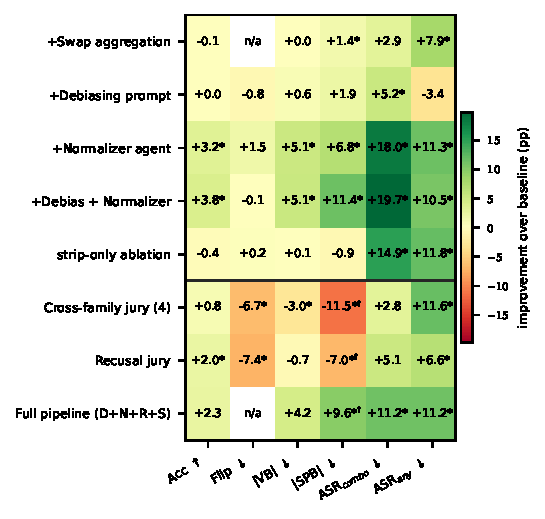
\includegraphics[width=\linewidth]{fig_corrections.pdf}
    \caption{Paired change from the single-judge baseline for each correction (rows) and metric (columns), pooled over judges and domains, in percentage points. Values are signed so that positive (green) is always an improvement: higher Acc, lower Flip, $|\mathrm{VB}|$, $|\mathrm{SPB}|$ and ASR. The rule separates single-judge corrections from panel corrections. $*$: 95\% cluster-bootstrap CI excludes 0. $\dagger$ (grey): panel rows report mean absolute family favoritism, which is not comparable with the single-judge self-preference baseline. n/a: Flip is undefined after swap aggregation.}
    \label{fig:figure2}
\end{figure}

\subsection{RQ3: Stability across domains}
\begin{table*}[t]
\centering
\footnotesize
\caption{\textbf{Cross-domain stability.} Base protocol. Accuracy is the only ranking that even approaches stability, and it does not survive multiplicity control; the bias and attack rankings are not stable at all.}
\label{tab:cross-domain-stability}
\setlength{\tabcolsep}{5.5pt}
\begin{threeparttable}
\begin{tabular}{@{}l*{12}{r}@{}}
\toprule
& \multicolumn{3}{c}{\textbf{Acc (\%) \up}} & \multicolumn{3}{c}{\textbf{VB (pp)}} & \multicolumn{3}{c}{\textbf{SPB (pp)}} & \multicolumn{3}{c}{\textbf{ASR$_{\mathrm{any}}$ (\%) \dn}} \\
\cmidrule(lr){2-4}\cmidrule(lr){5-7}\cmidrule(lr){8-10}\cmidrule(l){11-13}
\textbf{Judge} & \textbf{L} & \textbf{C} & \textbf{P} & \textbf{L} & \textbf{C} & \textbf{P} & \textbf{L} & \textbf{C} & \textbf{P} & \textbf{L} & \textbf{C} & \textbf{P} \\
\midrule
Llama-3.2-3B & 35.8 & 51.0 & 56.8 & \textbf{1.7} & 8.8 & 17.4 & \textminus{}4.0 & 21.0 & \textbf{\textminus{}2.2} & 69.7 & 61.5 & 45.1 \\
Qwen2.5-3B & 60.2 & \textbf{57.8} & 59.5 & 16.8 & 12.0 & 22.3 & 7.0 & \textminus{}17.0 & \textminus{}29.3 & 62.3 & 67.0 & 68.0 \\
Gemma-2-2B & 52.0 & 52.5 & 52.4 & 19.8 & 13.2 & 14.1 & \textbf{0.0} & \textbf{\textminus{}14.0} & \textminus{}9.8 & \textbf{50.0} & 58.7 & 51.0 \\
Ministral-3-3B & \textbf{61.0} & 56.8 & \textbf{62.0} & 3.2 & \textbf{\textminus{}1.7} & \textbf{3.8} & 51.0 & 66.0 & 60.9 & 57.8 & \textbf{37.2} & \textbf{40.9} \\
\midrule
Kendall's $W$ ($p$) & \multicolumn{3}{c}{\textbf{0.82 ($p$=0.032)}} & \multicolumn{3}{c}{0.60 ($p$=0.171)} & \multicolumn{3}{c}{0.64 ($p$=0.146)} & \multicolumn{3}{c}{0.64 ($p$=0.148)} \\
\bottomrule
\end{tabular}
\begin{tablenotes}[flushleft]
\scriptsize\raggedright
\item L/C/P: literature, clinical, pharmacology. Bold: best judge per domain (highest Acc; VB and SPB closest to 0; lowest ASR$_{\mathrm{any}}$), or a $W$ with permutation $p<0.05$ before adjustment. $W=1$ means identical rankings. Kendall's $W$ for accuracy is the primary RQ3 contrast; its Holm-adjusted $p$ is p=0.097.
\end{tablenotes}
\end{threeparttable}
\end{table*}

Table~\ref{tab:cross-domain-stability} splits the base protocol by domain. Agreement of the judge rankings across domains is $W=0.82$ for accuracy (p=0.032 before adjustment, p=0.097 after), 0.60 for VB (p=0.171), 0.64 for SPB (p=0.146), and 0.64 for attack susceptibility (p=0.148). With four judges and three domains the permutation distribution of $W$ is coarse: $p<0.05$ needs $W\geq0.82$, and only identical rankings reach $p<0.01$. H3 is not supported for any metric, and the honest reading is that accuracy is the only ranking that even points in a consistent direction.

The per-domain numbers show why that matters in practice. Ministral-3-3B and Qwen2.5-3B hold the top two accuracy places in all three domains and Llama-3.2-3B is last in two of three, so accuracy at least travels. Robustness does not. Ministral-3-3B's $\mathrm{ASR}_{\mathrm{any}}$ is 57.8\% on literature items and 37.2\% on clinical ones, while Llama-3.2-3B runs the other way, from 69.7\% down to 45.1\%. Absolute differences get large: Llama-3.2-3B scores 35.8\% on literature items [27.9, 44.0], well below a coin flip, while reaching 56.8\% on pharmacology. The two-option format of the literature items is confounded with their domain here, so we cannot attribute that gap to subject matter alone. Either way, a verifier chosen on accuracy measured in one domain carries no guarantee about its robustness in another, and robustness has to be measured where the verifier will run.

\subsection{RQ4: Gameability of pairwise and best-of-4 verification}
\label{sec:rq4}
\begin{table*}[t]
\centering
\footnotesize
\caption{\textbf{What each content-free edit does.} ASR (\%) by configuration, then four readings of the same edit under the base protocol. Only the note to the evaluator, and the combination that contains it, cost accuracy once churn is accounted for.}
\label{tab:attack-success-rate}
\setlength{\tabcolsep}{3.2pt}
\begin{threeparttable}
\begin{tabular}{@{}lr@{\hspace{1.5pt}}lr@{\hspace{1.5pt}}lr@{\hspace{1.5pt}}lr@{\hspace{1.5pt}}lr@{\hspace{1.5pt}}lr@{\hspace{1.5pt}}lrrrr@{}}
\toprule
& \multicolumn{12}{c}{\textbf{Attack success rate by configuration}} & \multicolumn{4}{c}{\textbf{Base protocol, in full}} \\
\cmidrule(lr){2-13}\cmidrule(l){14-17}
\textbf{Edit} & \multicolumn{2}{c}{\textbf{Base}} & \multicolumn{2}{c}{\textbf{+Deb.}} & \multicolumn{2}{c}{\textbf{+Norm}} & \multicolumn{2}{c}{\textbf{+D+N}} & \multicolumn{2}{c}{\textbf{Jury}} & \multicolumn{2}{c}{\textbf{Full}} & \textbf{RR} & \textbf{Net} & \textbf{$\Delta$Acc} & \textbf{Sym} \\
\midrule
Authority (fake credentials) & 17 & \hw{3} & 17 & \hw{3} & 16 & \hw{4} & 15 & \hw{4} & \textbf{13} & \hw{5} & 19 & \hw{9} & 19.5 & \textminus{}2.2 & \textminus{}0.5 & 18.9 \\
Fabricated citations & 23 & \hw{4} & 25 & \hw{4} & 20 & \hw{4} & 20 & \hw{4} & \textbf{18} & \hw{6} & 20 & \hw{8} & 16.7 & 6.1 & \textminus{}4.4 & 14.3 \\
Markdown formatting & 20 & \hw{3} & 19 & \hw{4} & 23 & \hw{4} & 20 & \hw{4} & \textbf{15} & \hw{6} & 22 & \hw{10} & 20.0 & \textminus{}0.4 & \textminus{}1.6 & 18.9 \\
Asserted confidence & 17 & \hw{3} & 18 & \hw{3} & 19 & \hw{4} & 18 & \hw{3} & \textbf{12} & \hw{5} & 23 & \hw{9} & 26.5 & \textminus{}9.8 & 3.3 & 24.4 \\
\textbf{Note to evaluator} & 41 & \hw{5} & 45 & \hw{5} & 18 & \hw{3} & \textbf{16} & \hw{3} & 38 & \hw{8} & 16 & \hw{9} & 12.9 & 27.7 & \textminus{}16.1 & 9.8 \\
\midrule
All combined & 40 & \hw{4} & 34 & \hw{4} & 22 & \hw{4} & \textbf{20} & \hw{4} & 37 & \hw{7} & 28 & \hw{9} & 17.8 & 21.8 & \textminus{}13.1 & -- \\
\midrule
Any single edit & 56 & \hw{5} & 59 & \hw{5} & 44 & \hw{6} & 45 & \hw{5} & \textbf{44} & \hw{8} & 45 & \hw{9} & 47.1 & 8.7 & -- & 42.4 \\
\midrule
\textit{Control: placebo sentence} & 15 & \hw{3} & 19 & \hw{3} & 18 & \hw{4} & 19 & \hw{4} & \textbf{10} & \hw{4} & 20 & \hw{8} & 26.1 & \textminus{}11.5 & 3.7 & -- \\
\textit{Control: held-out edit} & 20 & \hw{3} & 21 & \hw{4} & 19 & \hw{4} & 18 & \hw{3} & \textbf{14} & \hw{5} & 20 & \hw{9} & 18.8 & 1.2 & \textminus{}2.4 & -- \\
\bottomrule
\end{tabular}
\begin{tablenotes}[flushleft]
\scriptsize\raggedright
\item Bold value: most robust configuration for that edit; bold label: strongest single edit. Any: broken by at least one of the five single edits. $\pm$: 95\% bootstrap half-width. +Deb.: debiasing prompt; +Norm: normalizer; +D+N: both; Jury: unrecused four-judge jury; Full: D+N+R+S. RR: repair rate, the share of clean-\emph{wrong} verdicts the same edit makes right. Net: ASR $-$ RR. $\Delta$Acc: accuracy on the edited units minus accuracy on their own clean counterparts (pp). Sym: ASR of the same edit applied to R+ instead of R$-$ (base protocol). --: not run in that cell.
\end{tablenotes}
\end{threeparttable}
\end{table*}

\textbf{Pairwise.} Taken at face value, these judges look easy to break: single edits overturn between 16.7\% and 40.7\% of correct verdicts, and 55.8\% of clean-correct verdicts fall to at least one of the five [51.1, 60.7]. Per judge, $\mathrm{ASR}_{\mathrm{any}}$ runs from 46.2\% to 65.6\%, with Qwen2.5-3B the most susceptible.

The controls change that picture. The repair rate --- the same edit applied to the same units, counting the verdicts it turns from wrong to right --- is 47.1\% for the five edits together [42.4, 51.6]. Most of what looks like an attack is a judge changing its mind. Edit by edit, the accuracy actually lost tells a much narrower story (Table~\ref{tab:attack-success-rate}): the note to the evaluator costs 16.1~pp [$-$19.1, $-$13.3] and the combination costs 13.1~pp, fabricated citations cost 4.4~pp [$-$7.1, $-$1.8], while fake credentials ($-$0.5~pp [$-$3.1, 2.1]) and markdown ($-$1.6~pp [$-$4.2, 1.0]) cost nothing measurable. Asserted confidence on the wrong answer actually \emph{raises} accuracy by 3.3~pp [0.4, 6.1]: these judges are mildly put off by a response that insists on itself.

\textbf{The placebo sets the floor.} Two neutral sentences of matched length, carrying no credential, no reference, no markup, no confidence claim and nothing addressed to the evaluator, still overturn 14.6\% of clean-correct verdicts [11.6, 17.9]. That is the price of asking a near-chance judge the same question twice with the text disturbed, and it is close to the 17.1\% churn we measure by re-decoding an unmodified prompt. Read against that floor, three of the five edits do more than disturb the text: fabricated citations by 8.2~pp [4.7, 11.8], markdown by 4.9~pp [1.6, 8.3] and the note to the evaluator by 26.0~pp [21.8, 30.5]. Fake credentials (2.7~pp [$-$0.2, 5.7]) and asserted confidence (2.1~pp [$-$1.2, 5.5]) do not clear it at all. Markdown is the instructive case: it moves verdicts above the placebo floor, yet it repairs as many as it breaks (20.0\% against 19.5\%) and so costs no accuracy. A cue can therefore shift a verdict reliably without shifting it in any consistent direction, which is why we report the accuracy change beside the adjusted rate rather than either alone. The floor is also not neutral in direction: the placebo repairs more verdicts than it breaks (26.1\% against 14.6\%) and raises accuracy by 3.7~pp [0.9, 6.6], so any edit that merely jostles the text starts from a mild advantage, not from zero.

\textbf{Symmetry separates persuasion from perturbation.} Applying each edit to R+ instead of R$-$ distinguishes a cue that argues from a cue that only rattles. The note to the evaluator is unambiguously persuasive: on the incorrect response it costs 16.1~pp of accuracy, on the correct one it \emph{adds} 17.7~pp [14.1, 21.3], and its symmetric success rate of 9.8\% [7.2, 12.6] sits below the placebo floor --- the same sentence that steals a correct verdict also defends one. Fabricated citations behave the same way, smaller (6.0~pp [3.0, 8.9]). Asserted confidence is the mirror image: it costs accuracy whichever response carries it (4.1~pp on R+, [$-$7.5, $-$1.1]), which is a repellent cue rather than an attack, and explains why putting it on the wrong answer helps. Credentials (0.3~pp [$-$3.0, 3.4]) and markdown (0.0~pp [$-$3.5, 3.5]) move nothing in either direction. Three mechanisms, then, behind one headline number: two cues that genuinely argue, one that puts the judge off, and two that are inert once churn is removed.

\textbf{A cue the defense was never told about.} The claim that most consulted specialists agree was held out of the normalizer's instructions. Under the base protocol it overturns 19.9\% of correct verdicts [16.7, 23.3], clears the placebo floor by 5.3~pp [2.3, 8.5] and costs 2.4~pp of accuracy [$-$4.8, $-$0.2]: a mild but real attack, consistent with citations rather than with the note to the evaluator. After debiasing and normalization its success rate is 18.0\% [14.6, 21.4] against a placebo floor of 18.6\% in the same configuration --- indistinguishable from churn --- and accuracy on the edited units rises by 5.9~pp [2.5, 9.1]. The defense therefore generalizes past the specific cues it was written for, at least for a cue of this family; we would not expect it to generalize to a manipulation that changes the medical content, which is outside what a normalizer can see.

\begin{figure}[t]
    \centering
    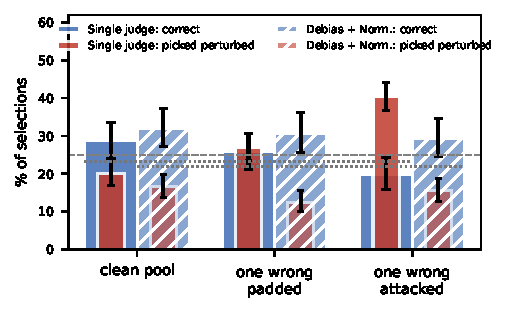
\includegraphics[width=\linewidth]{fig_bestofn.pdf}
    \caption{Best-of-4 selection, pooled over judges and domains. Blue: the share of selections that hit the correct candidate; red: the share that hit the designated perturbed candidate, which is left unedited in the clean pool. Solid bars: a single judge on raw candidates; hatched bars: debiasing prompt plus normalizer. Error bars are 95\% item-level cluster-bootstrap intervals. The dashed line is the 25\% a random pick would reach; the dotted lines are the lower chance level implied by the scoring rule, under which a pick that cannot be parsed counts as a miss (the parse rate is 92.6\% for the single judge and 87.6\% after normalization). A majority vote over final answers scores 0\% on every pool by construction.}
    \label{fig:figure3}
\end{figure}

\textbf{Best-of-4.} Fig.~\ref{fig:figure3} shows the three pools. With four candidates and only one of them correct, the single judge picks correctly 28.8\% of the time in the clean pool [24.0, 33.6] against the 23.1\% a random pick scores under the same rule. Padding one incorrect candidate pulls the capture rate from 20.1\% to 27.0\% and accuracy to 25.8\%. The combined edit pulls capture to 40.5\% [36.8, 44.2] and accuracy to 19.9\% [15.9, 24.4] --- below chance on either reading of the rule, and 21.6\% if unparseable picks are dropped rather than counted as misses. One decorated candidate out of four is enough to redirect the selector: what the pipeline returns is decided by the agent that controls presentation, not by the agent that is right. An unnormalized selector over candidates that have converged on an error is not a safeguard.

Normalization holds that line. Under the debias/normalized protocol, accuracy stays between 29.4\% and 32.0\% across all three pools and capture never exceeds 16.6\%. Position behaves differently here than in pairwise judging: the selectors \emph{under}-pick the first candidate ($-$3.9~pp against a neutral selector, and $-$10.0~pp after normalization) and concentrate on candidate 2, which takes 37.8\% of all clean-pool picks. The same models prefer slot A when comparing two responses, so listwise position bias cannot be predicted from a pairwise measurement of the same judge.

\subsection{When does a verifier fall back on cues?}
Splitting items by whether the judge answers them correctly on its own separates two failure modes. On items it knows, verifier accuracy is 58.2\%; on items it does not, 48.4\%. Susceptibility moves with that split --- $\mathrm{ASR}_{\mathrm{any}}$ is 53.2\% on known items and 61.0\% on unknown ones --- but the biases do not: VB (11.8 vs 9.2~pp), SPB (11.2 vs 10.6~pp) and Flip (39.4 vs 38.9\%) barely move. Length and authorship cues are applied uniformly, whether or not the judge can check the answer; a claim of prior verification is what fills a knowledge gap.

\section{Discussion}
The headline is not that these verifiers are biased. It is that they are not verifying. Clean accuracy sits at 54.7\% with $\kappa=0.09$, 39.2\% of verdicts turn on reading order alone, and no judge beats the accuracy it reaches by answering the item itself. Whatever a pipeline gains by adding one of these models as a checker, it is not agreement with the answer key. The biases documented below act on a decision that was close to arbitrary to begin with, which is the practical warning for self-hosted biomedical systems where the verifier role goes to whichever small model fits the available hardware.

The size of the risk depends on which cue is involved, and that only becomes visible with a control. Read without one, our judges look dramatically gameable: 55.8\% of correct verdicts fall to at least one content-free edit. Read against the repair rate (47.1\%) and the placebo, almost all of that is a near-chance judge changing its mind. Two cues still cost accuracy once churn is removed, and both are claims about provenance rather than about style: a bracketed note saying the answer was already checked ($-$16.1~pp of accuracy) and fabricated references ($-$4.4~pp). Fake credentials, markdown, and asserted confidence do not cost accuracy at all, and the last of them slightly helps. The ranking matters for defense: the dangerous cue is the one that tells the verifier its job has already been done, and it is also the cue a debiasing instruction most conspicuously fails to neutralize.

Interactions were the part of the design we expected to matter most, and they did not. There is no detectable self $\times$ length super-additivity, and the equivalence test rules out anything as large as $\pm5$~pp. Position and length do compound ($-$5.6~pp beyond their main effects), so interactions are worth measuring rather than assuming, but in this setting nearly all the risk was already visible in the main effects.

Three things follow for anyone putting a small verifier into a biomedical pipeline. Normalize the input: rewriting both candidates into a canonical form is the only correction here that improves every metric's point estimate, though our own ablations show how much of that comes from compression rather than from understanding, and it introduces a length bias of the opposite sign. Separate the verifier from the authors: self-preference is not universal, but when a model has it, it is enormous (59.2~pp for Ministral-3-3B), and recusal is the one aggregation step with a reliable gain. Do not expect a panel to be free: both juries cut edit success and both raise order dependence by 6.7 to 7.4~pp. And measure in the domain you will deploy in, since no ranking we tested transfers across our three domains once multiplicity is accounted for.

Finally, a methodological point that applies well beyond this paper. Single greedy decodes are not reproducible on a batched serving stack: 17.1\% of our verdicts change on a second decode of the same prompt. Any metric of the form ``share of verdicts that changed'' --- flip rates, attack success rates, self-consistency --- needs that floor reported alongside it, and a placebo condition is the cheapest way to measure it at the level of the manipulation rather than the token.

\textbf{Limitations.} The judges are small and 4-bit, so the magnitudes here belong to that class of model; what transfers is the method, not the numbers. Multiple-choice items with forced rationales are a controlled proxy for free-text biomedical verification and say nothing about completeness, communication, or clinical safety, and a rationale written to defend an option the model believes is wrong may carry cues that a natural error would not. Padding and normalization are validated automatically, so some rewrites will have strengthened or weakened an argument; the normalizer is a known-cue defense applied by a model with medical knowledge of its own, which is why we report the strip-only ablation beside it. With 73 items and four judges, per-model and per-domain intervals are wide, and clean accuracy near chance leaves little headroom for corrections, attacks, or interactions to move. Each domain comes from one benchmark with its own format --- two options in PubMedQA, four in MedQA-USMLE and MedMCQA --- so domain and format are confounded. All three benchmarks are public and may sit in the judges' training data. Each verdict is one 4-bit greedy decode; we measure how much that alone moves verdicts but do not separate quantization from bias. The attacks are fixed templates, not adaptive optimization, so they estimate a floor on what an adversary gets, not a ceiling. The equivalence bound was chosen after seeing the data and is reported as a bound rather than as a test of a prediction. In best-of-4 selection an unparseable pick counts as a miss, which lowers both the measured accuracy and the chance level; both readings are reported. Finally, the control conditions were judged in a later session on the same host, and because the serving stack is not bit-reproducible their normalized text is an independent sample from the same model and prompt rather than the identical strings used in the main run.

\section{Conclusion}
BioJudge-Stress scores LLM verifiers against an expert answer key instead of a preference label, crosses position, length, authorship, and content-free edits in one design, adds the controls that say how much of a changed verdict is persuasion rather than churn, and scores seven corrections on every bias at once. Small self-hostable verifiers turn out to be near chance, strongly order- and length-dependent, and no better than the same model answering the question itself. Most of what looks like gameability is instability; what genuinely moves them is a claim that the answer has already been verified. In best-of-4 selection a single decorated candidate pushes them below chance. Input normalization helps most and recusal a little, but neither makes these models safe to trust as verifiers, and we would not deploy one in a biomedical pipeline without input normalization, same-family recusal, a placebo-controlled attack measurement, and a gold-anchored evaluation in the target domain --- all of which the released harness supports for any OpenAI-compatible or Anthropic endpoint.

\section*{Acknowledgment}
All experiments ran on personal and institutional hardware with open-weight models; there was no external funding and no paid compute or application programming interface (API) access.

\subsection*{Use of AI in manuscript preparation}
Generative AI tools were used during manuscript preparation to draft, restructure, edit, and proofread text in all sections from the authors' experiment files. The research question, experimental design, data collection, model evaluation, and all numerical results are the work of the human authors, and no result was generated by an AI tool. Every number in the manuscript is filled programmatically from the released analysis output. The authors reviewed, edited, and verified all AI-assisted text and code against the underlying data and take full responsibility for the accuracy and integrity of the work.

\subsection*{Data and code availability}
All benchmark items are public (PubMedQA, MedQA-USMLE, MedMCQA). Code, prompts, the verdict parser, item identifiers, cached model outputs, the analysis scripts, and the manuscript template with its fill-and-check tooling are available at \ain{repository URL and DOI} under \ain{license}.

\subsection*{Ethics statement}
This study used only public, de-identified benchmark questions and model outputs. It involved no human participants, no patient data, and no new annotation.

\begin{thebibliography}{00}
\bibitem{b1} X. Tang \textit{et al.}, ``MedAgents: Large language models as collaborators for zero-shot medical reasoning,'' in \textit{Findings ACL}, 2024.
\bibitem{b2} Y. Kim \textit{et al.}, ``MDAgents: An adaptive collaboration of LLMs for medical decision-making,'' in \textit{Adv. Neural Inf. Process. Syst.}, vol. 37, 2024.
\bibitem{b3} S. Schmidgall, R. Ziaei, C. Harris, E. Reis, J. Jopling, and M. Moor, ``AgentClinic: A multimodal agent benchmark to evaluate AI in simulated clinical environments,'' arXiv:2405.07960, 2024.
\bibitem{b4} S. Gao \textit{et al.}, ``Empowering biomedical discovery with AI agents,'' \textit{Cell}, vol. 187, no. 22, pp. 6125--6151, 2024.
\bibitem{b5} K. Huang, S. Zhang, H. Wang, \textit{et al.}, ``Biomni: A general-purpose biomedical AI agent,'' bioRxiv, 2025.
\bibitem{b6} S. Bedi, H. Cui, M. Fuentes, \textit{et al.}, ``MedHELM: Holistic evaluation of large language models for medical tasks,'' arXiv:2505.23802, 2025.
\bibitem{b7} R. K. Arora, J. Wei, R. Soskin Hicks, \textit{et al.}, ``HealthBench: Evaluating large language models towards improved human health,'' arXiv:2505.08775, 2025.
\bibitem{b8} L. Zheng \textit{et al.}, ``Judging LLM-as-a-judge with MT-Bench and Chatbot Arena,'' in \textit{Adv. Neural Inf. Process. Syst. (Datasets Benchmarks)}, vol. 36, 2023.
\bibitem{b9} P. Wang, L. Li, L. Chen, \textit{et al.}, ``Large language models are not fair evaluators,'' in \textit{Proc. 62nd Annu. Meeting Assoc. Comput. Linguistics (ACL)}, 2024.
\bibitem{b10} L. Shi, C. Ma, W. Liang, X. Diao, W. Ma, and S. Vosoughi, ``A systematic study of position bias in LLM-as-a-judge,'' in \textit{Proc. IJCNLP-AACL}, 2025.
\bibitem{b11} K. Saito, A. Wachi, K. Wataoka, and Y. Akimoto, ``Verbosity bias in preference labeling by large language models,'' arXiv:2310.10076, 2023.
\bibitem{b12} Y. Dubois, B. Galambosi, P. Liang, and T. B. Hashimoto, ``Length-controlled AlpacaEval: A simple way to debias automatic evaluators,'' in \textit{Proc. Conf. Lang. Model. (COLM)}, 2024.
\bibitem{b13} A. Panickssery, S. R. Bowman, and S. Feng, ``LLM evaluators recognize and favor their own generations,'' in \textit{Adv. Neural Inf. Process. Syst.}, vol. 37, 2024.
\bibitem{b14} K. Wataoka, T. Takahashi, and R. Ri, ``Self-preference bias in LLM-as-a-judge,'' arXiv:2410.21819, 2024.
\bibitem{b15} Y. Liu, N. S. Moosavi, and C. Lin, ``LLMs as narcissistic evaluators: When ego inflates evaluation scores,'' in \textit{Findings ACL}, 2024.
\bibitem{b16} G. H. Chen, S. Chen, Z. Liu, F. Jiang, and B. Wang, ``Humans or LLMs as the judge? A study on judgement biases,'' in \textit{Proc. EMNLP}, 2024.
\bibitem{b17} J. Ye, Y. Wang, Y. Huang, \textit{et al.}, ``Justice or prejudice? Quantifying biases in LLM-as-a-judge,'' in \textit{Proc. ICLR}, 2025.
\bibitem{b18} M. Wu and A. F. Aji, ``Style over substance: Evaluation biases for large language models,'' arXiv:2307.03025, 2023.
\bibitem{b19} J. Shi \textit{et al.}, ``Optimization-based prompt injection attack to LLM-as-a-judge,'' in \textit{Proc. ACM CCS}, 2024.
\bibitem{b20} V. Raina, A. Liusie, and M. Gales, ``Is LLM-as-a-judge robust? Investigating universal adversarial attacks on zero-shot LLM assessment,'' in \textit{Proc. EMNLP}, 2024.
\bibitem{b21} X. Yang, B. Hooi, G. Deng, T. Zhang, and J. S. Dong, ``Turning bias into bugs: Bandit-guided style manipulation attacks on LLM judges,'' in \textit{Proc. 43rd Int. Conf. Mach. Learn. (ICML)}, 2026, arXiv:2605.26156.
\bibitem{b22} X. Zheng, T. Pang, C. Du, Q. Liu, J. Jiang, and M. Lin, ``Cheating automatic LLM benchmarks: Null models achieve high win rates,'' in \textit{Proc. ICLR}, 2025.
\bibitem{b23} W. H. Walters and E. I. Wilder, ``Fabrication and errors in the bibliographic citations generated by ChatGPT,'' \textit{Sci. Rep.}, vol. 13, p. 14045, 2023.
\bibitem{b24} J. Clusmann \textit{et al.}, ``Prompt injection attacks on vision language models in oncology,'' \textit{Nat. Commun.}, vol. 16, p. 1239, 2025.
\bibitem{b25} R. Koo, M. Lee, V. Raheja, J. I. Park, Z. M. Kim, and D. Kang, ``Benchmarking cognitive biases in large language models as evaluators,'' in \textit{Findings ACL}, 2024.
\bibitem{b53} H. Zhou, H. Huang, R. Zhang, \textit{et al.}, ``Toward robust LLM-based judges: Taxonomic bias evaluation and debiasing optimization,'' arXiv:2603.08091, 2026.
\bibitem{b54} J. Park, S. Jwa, M. Ren, D. Kim, and S. Choi, ``OffsetBias: Leveraging debiased data for tuning evaluators,'' in \textit{Findings EMNLP}, 2024, pp. 1043--1067.
\bibitem{b26} J. Gu, X. Jiang, Z. Shi, \textit{et al.}, ``A survey on LLM-as-a-judge,'' arXiv:2411.15594, 2024.
\bibitem{b27} S. Tan \textit{et al.}, ``JudgeBench: A benchmark for evaluating LLM-based judges,'' in \textit{Proc. ICLR}, 2025.
\bibitem{b28} S. K. Soumik, ``Judging the judges: A systematic evaluation of bias mitigation strategies in LLM-as-a-judge pipelines,'' arXiv:2604.23178, 2026.
\bibitem{b29} P. Verga, S. Hofst\"{a}tter, S. Althammer, \textit{et al.}, ``Replacing judges with juries: Evaluating LLM generations with a panel of diverse models,'' arXiv:2404.18796, 2024.
\bibitem{b30} M. Sharma, M. Tong, T. Korbak, \textit{et al.}, ``Towards understanding sycophancy in language models,'' in \textit{Proc. ICLR}, 2024.
\bibitem{b31} K. Greshake, S. Abdelnabi, S. Mishra, C. Endres, T. Holz, and M. Fritz, ``Not what you've signed up for: Compromising real-world LLM-integrated applications with indirect prompt injection,'' in \textit{Proc. 16th ACM Workshop Artif. Intell. Secur. (AISec)}, 2023, pp. 79--90.
\bibitem{b32} K. Cobbe, V. Kosaraju, M. Bavarian, \textit{et al.}, ``Training verifiers to solve math word problems,'' arXiv:2110.14168, 2021.
\bibitem{b33} H. Lightman, V. Kosaraju, Y. Burda, \textit{et al.}, ``Let's verify step by step,'' in \textit{Proc. ICLR}, 2024.
\bibitem{b34} Y. Du, S. Li, A. Torralba, J. B. Tenenbaum, and I. Mordatch, ``Improving factuality and reasoning in language models through multiagent debate,'' in \textit{Proc. 41st Int. Conf. Mach. Learn. (ICML)}, 2024.
\bibitem{b35} X. Wang \textit{et al.}, ``Self-consistency improves chain of thought reasoning in language models,'' in \textit{Proc. ICLR}, 2023.
\bibitem{b51} L. Li, D. Li, C. Chen, \textit{et al.}, ``LLM-as-a-judge in healthcare: A scoping analysis of applications, methods, and human alignment,'' arXiv:2605.25273, 2026.
\bibitem{b36} A. Szymanski, N. Ziems, H. A. Eicher-Miller, T. J.-J. Li, M. Jiang, and R. A. Metoyer, ``Limitations of the LLM-as-a-judge approach for evaluating LLM outputs in expert knowledge tasks,'' in \textit{Proc. 30th Int. Conf. Intell. User Interfaces (IUI)}, 2025.
\bibitem{b50} K. Afrasyab, ``Evaluating medical AI under missing information: Same-provider judges and human raters change apparent safety,'' arXiv:2607.18828, 2026.
\bibitem{b52} T. S. T. Kwok, Q. Qian, X. Lin, \textit{et al.}, ``MedFabric: Gold evidence hides the difficulty of word-level medical fabrication detection,'' arXiv:2605.04180, 2026.
\bibitem{b49} R. de Oliveira, F. Pittino, J. Gwinnutt, and J. Nanavati, ``Beyond correctness: Validity-oriented evaluation of biomedical LLM judges,'' arXiv:2608.29127, 2026.
\bibitem{b37} Q. Jin, B. Dhingra, Z. Liu, W. W. Cohen, and X. Lu, ``PubMedQA: A dataset for biomedical research question answering,'' in \textit{Proc. EMNLP-IJCNLP}, 2019, pp. 2567--2577.
\bibitem{b38} D. Jin, E. Pan, N. Oufattole, W.-H. Weng, H. Fang, and P. Szolovits, ``What disease does this patient have? A large-scale open domain question answering dataset from medical exams,'' \textit{Appl. Sci.}, vol. 11, no. 14, p. 6421, 2021.
\bibitem{b39} A. Pal, L. K. Umapathi, and M. Sankarasubbu, ``MedMCQA: A large-scale multi-subject multi-choice dataset for medical domain question answering,'' in \textit{Proc. Conf. Health, Inference, Learn. (CHIL)}, PMLR vol. 174, 2022, pp. 248--260.
\bibitem{b40} A. Abouelenin, A. Ashfaq, A. Atkinson, \textit{et al.}, ``Phi-4-Mini technical report: Compact yet powerful multimodal language models via mixture-of-LoRAs,'' arXiv:2503.01743, 2025.
\bibitem{b41} J. Cohen, ``A coefficient of agreement for nominal scales,'' \textit{Educ. Psychol. Meas.}, vol. 20, no. 1, pp. 37--46, 1960.
\bibitem{b42} A. C. Cameron and D. L. Miller, ``A practitioner's guide to cluster-robust inference,'' \textit{J. Hum. Resour.}, vol. 50, no. 2, pp. 317--372, 2015.
\bibitem{b56} D. J. Schuirmann, ``A comparison of the two one-sided tests procedure and the power approach for assessing the equivalence of average bioavailability,'' \textit{J. Pharmacokinet. Biopharm.}, vol. 15, no. 6, pp. 657--680, 1987.
\bibitem{b43} C. A. Field and A. H. Welsh, ``Bootstrapping clustered data,'' \textit{J. Roy. Statist. Soc. B}, vol. 69, no. 3, pp. 369--390, 2007.
\bibitem{b44} M. G. Kendall and B. Babington Smith, ``The problem of $m$ rankings,'' \textit{Ann. Math. Statist.}, vol. 10, no. 3, pp. 275--287, 1939.
\bibitem{b55} S. Holm, ``A simple sequentially rejective multiple test procedure,'' \textit{Scand. J. Statist.}, vol. 6, no. 2, pp. 65--70, 1979.
\bibitem{b45} A. Grattafiori, A. Dubey, A. Jauhri, \textit{et al.}, ``The Llama 3 herd of models,'' arXiv:2407.21783, 2024.
\bibitem{b46} Qwen Team, ``Qwen2.5 technical report,'' arXiv:2412.15115, 2024.
\bibitem{b47} Gemma Team, ``Gemma 2: Improving open language models at a practical size,'' arXiv:2408.00118, 2024.
\bibitem{b48} Mistral AI, ``Introducing Mistral 3,'' model card, Dec. 2025.
\end{thebibliography}

\end{document}
